\documentclass[11pt]{p9article}
\usepackage{epsfig}

\textheight	230mm 
\textwidth 150mm
\topmargin +5mm
\oddsidemargin 0mm
\evensidemargin 0mm

\setlength\parindent{0pt}
\setlength\parskip{0.25\baselineskip}

\renewcommand\baselinestretch{0.8}
\renewcommand{\familydefault}{\sfdefault}

\makeatletter
\renewcommand\section{\@startsection {section}{1}{\z@} {3pt} {1pt} {\normalfont\normalsize\bfseries}}
\renewcommand\subsection{\@startsection {subsection}{1}{\z@} {3pt} {1pt} {\normalfont\normalsize\bfseries}}
\makeatother

\begin{document}
\title{\Large\textbf{The Xcpu Cluster Management Framework}}
\author{\large 
	\begin{tabular}{c}
	\textsl{Latchesar Ionkov, Ron Minnich, Andrey Mirtchovski}\\
	\textsl{Los Alamos National Laboratory\footnote{LANL publication: LA-UR-06-7798}}\\
	\texttt{\{lionkov,rminnich,andrey\}@lanl.gov}\\
	\end{tabular}
}

\maketitle\thispagestyle{empty}
\pagestyle{empty}

\begin{abstract}

\setlength\parindent{0pt}
\setlength\parskip{0.25\baselineskip}

This paper describes the organization and implementation of the
Xcpu cluster management framework currently in use at the Los Alamos
National Laboratory. Xcpu is used to start, monitor and control
jobs on a variety of remote nodes in a cluster environment. Xcpu
can be used for computation both on lightweight nodes with no local
storage as well as full-blown installations of various operating
systems. It is portable amongst all UNIX and UNIX-like operating
systems. Xcpu has been optimized to scale to hundreds and thousands
of nodes.
\end{abstract}

\section{Introduction} 
Xcpu is a remote process execution system that represents execution
and control services as a set of files in a hierarchical file system.
The file system can be exported and mounted  remotely over the
network.  Xcpu is slated to replace the aging B-proc~\cite{choi-life}
cluster management suite and xcpu is portable across all UNIX and
UNIX-like operating systems; an implementation exists for the Plan
9~\cite{pike95plan} operating system as well. Our current Xcpu
implementation is written in C, however there are no restrictions
to the languages that it could be implemented with. We have heard
at least of one more implementation of an earlier specification
written in the language Limbo~\cite{limbo} for the Inferno~\cite{inferno}
operating system. Xcpu has been designed to run on a variety of
size machines, scaling to thousands of computational nodes~\cite{1019813},
if proper security mechanisms are implemented, such as the ones
that exist for the Plan 9 operating system~\cite{cox02security},
Xcpu may be used for wide-area computational environments such as
grids~\cite{mirtchovski04grid}.

A cluster that uses Xcpu has one or more control nodes. The control
nodes represent the global view of the cluster and can be used to
execute, view and control of distributed programs. The rest of the
cluster nodes known as compute nodes and are used to run distributed
applications as guided by the control node.

Xcpu is responsible not only for the execution of the programs, but
also for their distribution to the compute nodes. It allows an
arbitrary number of files (shared libraries, configuration files, etc.)
to be pushed with the executable. In order to avoid the network
bandwidth bottleneck between the control node and the compute nodes,
Xcpu uses some of the compute nodes for the program distribution
by dedicating them as distribution nodes for the duration of the
program startup. This scheme, borrowed from B-proc, decreases
significantly the start-up time for distributed applications.

\section{Client Interaction}
The use of a standard file-system interface makes the system easy
to understand and easy to work with since
files are a well understood concept both at the user and at the
programmatic level. Furthermore, the ability to mount a compute
node over the network to the local file system is a significant
departure from the antiquated ``remote execution'' model in which
little or no control over the application is given to the end user.

A session with an Xcpu server consists of opening files, writing
to them and reading results. Several files correspond to the major
communication paths in UNIX, namely \textsl{stdin}, \textsl{stdout}
and \textsl{stderr}, a few other files deal with control over the
session and the environment it runs in, yet a few more provide information about the running
state of the computational node. All these are explained in subsequent
sections.  Below is a sample session to an Xcpu compute node which launches
a single process and displays its output on the console:
\begin{verbatim}
	$ mount -t 9p 192.168.100.101 /mnt/xcpu/1 -o port=666
	$ cd /mnt/xcpu/1
	$ ls -l
	total 0
	-r--r--r-- 1 root root 0 Jul 25 10:19 arch
	-r--r--r-- 1 root root 0 Jul 25 10:19 clone
	-rw-r--r-- 1 root root 0 Jul 25 10:19 env
	-r--r--r-- 1 root root 0 Jul 25 10:19 procs
	-r--r--r-- 1 root root 0 Jul 25 10:19 uname
	$ tail -f clone &
	[1] 8237
	0tail: clone: file truncated
	$ cd 0
	$ ls -l
	total 0
	-rw-rw-rw- 1 nobody nobody 0 Jul 25 12:58 argv
	-rw-rw-rw- 1 nobody nobody 0 Jul 25 12:58 ctl
	-rw-rw-rw- 1 nobody nobody 0 Jul 25 12:58 env
	-rw-rw-rw- 1 nobody nobody 0 Jul 25 12:58 exec
	drwx------ 1 nobody nobody 0 Jul 25 12:58 fs
	-r--r--r-- 1 nobody nobody 0 Jul 25 12:58 state
	-r--r--r-- 1 nobody nobody 0 Jul 25 12:58 stderr
	-rw-rw-rw- 1 nobody nobody 0 Jul 25 12:58 stdin
	-rw-rw-rw- 1 nobody nobody 0 Jul 25 12:58 stdio
	-r--r--r-- 1 nobody nobody 0 Jul 25 12:58 stdout
	-rw-rw-rw- 1 nobody nobody 0 Jul 25 12:58 wait
	$ cp /bin/date fs
	$ echo exec date > ctl
	$ cat stdout 
	Tue Jul 25 12:59:11 MDT 2006
	$
\end{verbatim}

The communication steps required for successfully executing a session
are as follows: the xcpufs file system is mounted at \verb|/mnt/xcpu/1|.
Reading from the \verb|clone| file creates a new session on the server and returns
its ID. The user can copy an arbitrary number of files to the
\verb|fs| directory. The execution of the program is done by writing
\verb|exec |{\sl progname} to \verb|ctl| file.

\section{Xcpufs}
Xcpufs is a file server that runs on all compute nodes and exports an
interface for program execution and control as a file hierarchy. The file
server uses Plan9's 9P2000~\cite{9p}~\cite{graverobbers} protocol. Xcpufs can be mounted on a Linux
control node using v9fs~\cite{minnich-vfs}~\cite{v9fseric}, or can be accessed directly using clients that
speak 9P2000.

Xcpufs manages the processes it executes in sessions. In order to execute a
program, the user creates a session, copies all required files, including
the executable, sets up the argument list and the program environment and
executes the program. The user can send data to program's standard input,
read from its standard output and error, and send signals.

Only one program can be executed per session. The process of this program is
known as {\sl main session process}. That process may spawn other processes
on the compute node. Xcpufs can control (send signals, destroy) only the
main session process. 

There are two types of sessions -- normal and persistent. The {\sl normal}
session (and the subdirectory that represents it) exists as long as there is
an open file in the session directory, or the main session process is
running. The {\sl persistent} session doesn't disappear unless the user
manually {\sl wipes} it. 

Normally the program will run as the user that attached the filesystem
(field \verb|uname| in Tattach 9P2000 message). The program can be executed
as somebody else if the ownership of the session subdirectory is changed to
different user. The files in the session directory are accessible by the
owner and the members of the owners default group.

All files that are copied to a session are stored in a temporary directory
on the compute node. Before executing the program, xcpufs changes the
process' current directory to the session directory, and sets the \textbf{XCPUPATH}
envrironment variable to point to it. All files in the temporary storage are
deleted when the session is destroyed.

In addition to the environment set through the env file, xcpufs adds three
more variables:

\begin{description}

\item[XCPUPATH] contains the full path to session's temprary directory
\item[XCPUID] contains the global ID of the session (same as the {\tt id} file)
\item[XCPUSID] contains the local session ID (same as the session directory)

\end{description}

\section{File Hierarchy of Xcpu Servers}
The file hierarchy of Xcpu servers consists of two main parts, a
top-level directory and one or more directories corresponding to
established sessions to that server by clients. The top-level
directory of the file server contains several files which hold
information about the machine which the server is running on, its
status and the currently running processes on it. The non-directory
files in the xcpufs root are:

\begin{verbatim}
        arch
        clone
        env
        procs
        state
\end{verbatim}

\verb|Arch| is a read-only file, reading from it returns the architecture of
the compute node in a format {\sl operating-system/processor-type}.

\verb|Clone| is a read-only file. When it is opened, xcpufs creates a new
session and exports a new session directory in the file-system. It also
copies the content of the global \verb|env| file to the session one. The
open can fail if the content of the global \verb|env| file is not formatted
correctly. 

Reading from the file returns the name of the session directory. 

\verb|Env| contains the global environment to be used for all new sessions.
When a new session is created, the content of \verb|env| is copied to the
sessions \verb|env| file.

Reading from the file returns the current environment. Writing to the file
changes the environment. 

The content of the global and session environment files have the following
format:

\begin{verbatim}
	environment = *env-line
	env-line = env-name ``='' env-value LF
	env-name = ALPHA *[ALPHA | DIGIT]
	env-value = ANY
\end{verbatim}

If the \verb|env-value| contains whitespace characters (SP, TAB or LF) or
single quotes, it is enclosed in single quotes and the original single
quotes are doubled (i.e. \verb|'| becomes \verb|''|).

\verb|Procs| is a read-only file. The content of the file is a s-expression~\cite{sexpr}
that list all processes running on the compute node. The first subexpression
contains list of the fields returned for the processes. The list is
architecture dependent.

\verb|State| file contains the state of the node. The user can write any
string to the file.  

\section{Session directory}
The session directory contains files pertaining to a particular
user session. These files provide interfaces for control of the
execution of the program, the environment which it runs in, pointers
to local storage in which to put libraries and extra files needed
for the execution, as well as files containing the standard input
and output for the program. The files and directories of a session are described below.

\begin{verbatim}
        argv
        ctl
        exec
        env
        fs
        state
        stdin
        stdout
        stderr
        stdio
        wait
        id
\end{verbatim}

\subsection{{\tt Ctl} file}

The \verb|ctl| file is used to execute and control session's main process.

Reading from the file returns the main process pid if the process is running
and -1 otherwise.

The operations on the session are performed by writing to it. \verb|Ctl|
commands have the following format:

\begin{verbatim}
	ctl = *cmd-line
	cmd-line = command `` `` *[argument] LF
	command = ``exec'' | ``clone'' | ``wipe'' | 
		  ``signal'' | ``close'' | ``type''
	argument = ANY
\end{verbatim}

If the \verb|argument| contains whitespace characters (SP, TAB or LF) or single
quotes, it is enclosed in single quotes and the original single quotes are
doubled (i.e. \verb|'| becomes \verb|''|).

Writing to \verb|ctl| ignores the specified offset and always appends the
data to the end of the file. It is not necessary a write to contain a whole
(or single) command line. Xcpufs appends the current write data to the end
of the buffer, and executes all full command lines. The write operation
returns when all valid commands are finished.

\verb|Ctl| supports the following commands:

\begin{description}

\item[exec {\sl program-name} {\sl directory} ] Execute the program. For
backward compatibility, if program name is not specified, xcpufs executes
the program named ``xc'' from the session directory. If the {\sl directory}
is specified, xcpufs sets the current directory to that value before
executing the binary. If it is not specified, the session directory is used.

If the program-name is a relative path (i.e. doesn't start with `/'
character, the session directory path is appended in front of it.

\item[clone {\sl max-sessions address-list}] Copies the current session content
(argument list, environment and files from \verb|fs| directory) to the
specified sessions. If \verb|max-sessions| is greater than zero, and the
number of the specified sessions is bigger than \verb|max-sessions|,
\verb|clone| pushes its content to up to max-sessions and issues
\verb|clone| commands to some of them to clone themselves to the remaining
sessions from the list.

The format of the session-address is:

\begin{verbatim}
	address-list = 1*(session-address ``,'')
	session-address = [``tcp!''] node-name [``!''port] 
		          ``/'' session-id
	node-name = ANY
	port = NUMBER
	session-id = ANY
\end{verbatim}

\item [wipe] Closes the standard I/O files, if the main session process is
still alive, kills it (SIGTERM) and frees all objects used by the session.
This command is normally used to terminate persistent sessions. 

\item [signal {\sl sig}] Sends a signal to the main session process. The
signal can be specified by number, or name. The supported signal names may
depend on the node's architecture.

\item [type {\tt normal} $|$ {\tt persistent}] Changes the type of the session.

\item [close {\tt stdin} $|$ {\tt stdout} $|$ {\tt stderr}] Closes the
standard input/output/error of the main session process.

\item [id {\sl id}] Sets the session id (see the \verb|id| file). If the
job-id or the proc-id parts are ommited, they are not changed.

\end{description}

Reading from the \verb|ctl| file returns the session ID. 

Sending a signal to a session that doesn't have running process will cause
the write function to return an error.

\subsection{{\tt Exec} file}

The exec file is kept for backward compatibility. Writing to it creates a
file named ``exec'' in the \verb|fs| directory.

\subsection{{\tt Fs} directory}

The \verb|fs| directory points to the temporary storage created for the
session. The user can create directories and files in that directory.
Creation of special files (symbolic links, devices, named pipes) is not
allowed. 

\subsection{{\tt Argv} file}

Writing to the \verb|argv| file sets the program argument list. 

\verb|argv| has the following format:

\begin{verbatim}
	argument-list = 1*(argument (SP | TAB | LF))
	argument = ANY
\end{verbatim}

If the \verb|argument| contains whitespace characters (SP, TAB or LF) or single
quotes, it is enclosed in single quotes and the original single quotes are
doubled (i.e. \verb|'| becomes \verb|''|).

Reading from the \verb|argv| file returns the current content.

\subsection{{\tt Env} file}

When the session is created, the content of the \verb|env| file is populated
from the global \verb|env| file.

Writing to the \verb|env| file modifies the session environment.
Modifications done after the program is executed don't change its
environment.

The format of the session \verb|env| file is identical to the global one.

\subsection{{\tt State} file}

\verb|State| is a file that can be used both for reading and
writing. It is used by the cluster monitoring framework to mark
computational nodes' states. When Xcpu starts the state file contains
no information. If a string is written to it this string is returned
by subsequent reads.

\subsection{{\tt Stdin} file}

\verb|Stdin| is a write-only file. The data from the write operation is
passed to the standard input of the main session process. The write may
block if the main process doesn't consume the data.

Closing the stdin file doesn't close the standard input stream of the
main process. The file can safely be opened and closed multiple times.

\subsection{{\tt Stdout} file}

\verb|Stdout| is a read-only file. The read operations blocks until the main
session process writes some data to its standard output.

If the file is opened more than once, and there are blocked read
operations for these files when some data is available from the standard
output, xcpufs sends the data to every open file.

Closing the \verb|stdout| file doesn't close the standard output stream of the
main process. The file can safely be opened and closed multiple times.

\subsection{{\tt Stderr} file}

\verb|Stderr| is a read-only file. The read operations blocks until the main
session process writes some data to its standard error.

If the file is opened more than once, and there are blocked read
operations for these files when some data is available from the standard
output, xcpufs sends the data to every open file.

Closing the \verb|stderr| file doesn't close the standard output stream of the
main process. The file can safely be opened and closed multiple times.

\subsection{{\tt Stdio} file}

\verb|Stdio| file combines \verb|stdin| and \verb|stdout| functions.
Reading from \verb|stdio| is equivalent to reading from \verb|stdout|, and
writing to it is equivalent to writing to \verb|stdin|.

If the file is opened more than once, and there are blocked read
operations for these files when some data is available from the standard
output, xcpufs sends the data to every open file.

\subsection{{\tt Wait} file}

\verb|Wait| is a read-only file. Reading from it returns the exit code of
the main session process. The read operations will block until the process
ends.

\subsection{{\tt Id} file}

\verb|Id| is a read-only file that contains the user-specified id. The
format of the id is:

\begin{verbatim}
	id = job-id ``/'' proc-id
	job-id = ANY
	proc-id = NUMBER
\end{verbatim}

The job-id is a global identifier of the job, the proc-id is an id of the
process within the job. Both are set by the user via ``id'' command.

\section{Monitoring of Xcpu Clusters}
\subsection{StatFS}
Our main monitoring tool for Xcpu clusters is \textit{Statfs}.
Statfs is a file server which connects to a set of Xcpu nodes and
reports their status through its various files. Currently Statfs
serves the following files: 

\begin{description} 
\item [\texttt{ctl}] This file accepts commands to statfs which cause it to quit or
reload the configuration file
\item [\texttt{notify}] This file can be used for notifications of
change in status for file servers. A read to this file will block
until a node or several nodes have changed status
\item [\texttt{state}] Reading this file returns a whitespace-separated
list of node, architecture, ip address and status. Each line
corresponds to a single node. Note that this is a departure from
the s-expression~\cite{sexpr} method of data reporting accepted elsewhere. This
is a problem with the current system which we are addressing.
\end{description} 

Statfs currently uses a configuration file which
it reads at startup or whenever the \textbf{reconfigure} command
is issued to the \texttt{ctl} file. This configuration file contains
information about the compute nodes which Statfs should report
information for. The format for this file is as follows:
\begin{verbatim}
        x1=tcp!127.0.0.1!2000
        x2=tcp!127.0.0.1!2001
        x3=tcp!127.0.0.1!2002
        x4=tcp!127.0.0.1!2003
\end{verbatim}
Each line corresponds to a single node. The first element is the
name of the node, also what it may be mounted as under \texttt{/mnt/xcpu}
for systems which use v9fs to mount compute nodes. The second element
is a standard Plan 9 \texttt{dial()}~\cite{presottonetworks} string.
In the future we would expect Xcpu compute nodes to be able to
announce themselves to Statfs for automatic configuration of live
clusters and grids. We would also consider converting the configuration
file format to s-expressions to fit better with the rest of the
system.


\subsection{Mongo}
Mongo is a new distributed cluster monitoring framework designed
to be deployed on several of the High Performance Computing clusters
here at Los Alamos National Laboratory. Mongo's design borrows ideas
from our previous monitoring network for B-Proc clusters:
Supermon.~\cite{supermon} The Mongo architecture allows us to
hierarchically monitor and control the data gathering of various
monitoring services, from kernel performance counters to system
logs.

Mongo is designed to perform on a variety of systems in a variety
of configurations: from the local desktop to a cluster of thousands
of compute nodes such as Coyote, at LANL. If paired with an
authentication and security mechanisms such as the ones available
for grids such as 9grid, the Mongo architecture can be extended to
provide monitoring for distributed environments that span administrative
domains.

The Mongo architecture employs two types of servers: node monitors
(mongos), and aggregators, which combine information from several
mongos into a single stream of data. Mongo is built around the 9P
communication protocol which allows both client and servers to
communicate via file operations. A mongo server presents a file
hierarchy of files containing measurements for a particular machine,
as well as files that can be used to control various aspects of the
measurement. Clients access those files to read data or to modify
the gathering methods. A sample arrangement of the Mongo architecture
is shown in Figure~\ref{graph:mongo}.

\begin{figure}[h]
\begin{center}
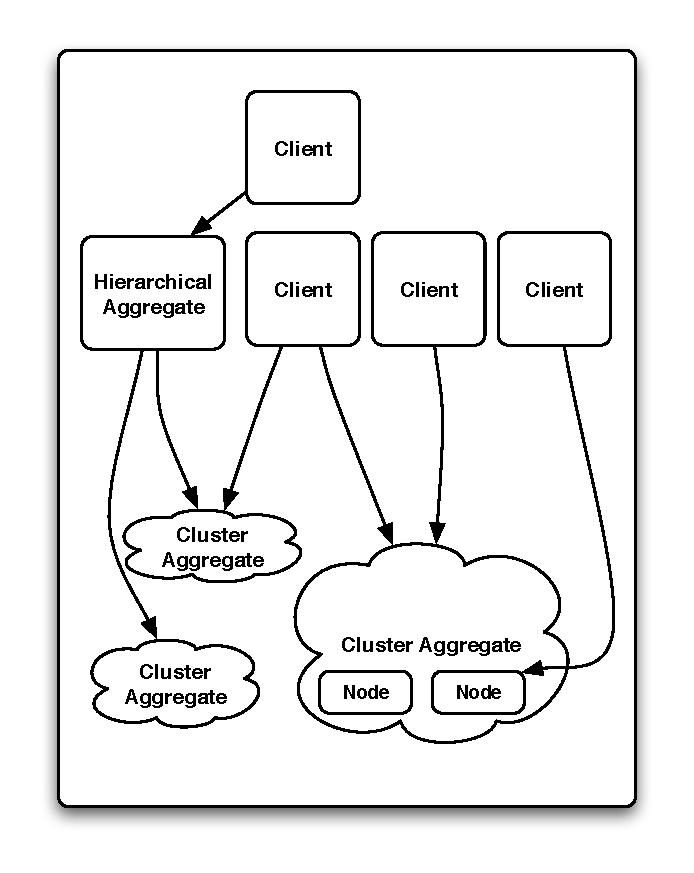
\includegraphics
        [height=8cm,keepaspectratio] 
        {mongo-fig1.eps}\\
\begin{minipage}{150mm}
\caption{ Several possible arrangements between
servers, aggregators and clients are available: clients can contact mongo
servers directly (given appropriate permissions) via 9P, or they
can attach to a cluster aggregate, which combines the data from
several compute nodes into a single stream without modifying it.} 
\label{graph:mongo}
\end{minipage}
\end{center}
\end{figure}

Since the data format we use, s-expressions, is recursive, information
from various aggregates can be combined together infinitely for
views of even larger scale, such as for example all the computational
units of a single organization, or a grid-like environment spanning
multiple organizations.  

Mongo employs both the push and pull model for data distribution
which sets it apart from other monitoring frameworks. By choosing
which file to read a client would either be notified of an event
(a read will block until a particular event has occurred) or will
read the current status of all monitored variables. We expect this
approach to scale significantly better on large number of monitored
nodes due to the possibility of a significantly finer-grained
filtering of the information gathered.

\section{Conclusions}
Xcpu has passed two protorype stages and is reaching maturity as a
full-fledged program. It is deployed on several of our development
clusters (around 100 nodes) and is being evaluated for larger
clusters at other LANL organizations. The performance metrics
gathered from the second prototype allow us to reach the conclusion
that the Xcpu model is not inherently slower than B-Proc. On test
runs of up to 800 nodes we were only a factor of 2 slower in start-up
time. While the current code base may be a bit slower due to it
being much more complete feature-wise, it is still within shouting
distance from our benchmark suite: B-Proc. It is important to note,
that the most important from a performance point of view measurements,
namely those of start-up time, control and teardown of large sessions
take significantly less time, often less than a percent of the total
running time for an application.

There is significant commercial interest in Xcpu from High-Performance
Computing companies and other scientific organizations. Both TerraSoft
and NASA are evaluating early versions of the Xcpu code.

\bibliography{xcpu-madrid}
\bibliographystyle{plain}

\end{document}
